\documentclass[aspectratio=1610,xcolor=dvipsnames,table]{beamer}


\xdefinecolor{darkgreen}{RGB}{000, 88, 000}
\xdefinecolor{greyblue}{RGB}{200, 200, 255}
\makeatletter
\newcommand*{\mylength}[1]{\strip@pt#1}
% Or rounded back to `cm` (there will be some rounding errors!)
%\newcommand*{\getlength}[1]{\strip@pt\dimexpr0.035146\dimexpr#1\relax\relax}

\makeatother

\mode<presentation>
{
  \usetheme{Luebeck}
%\usecolortheme[named=PineGreen]{structure}
\usecolortheme[named=gray]{structure}
  \setbeamercovered{invisible}
\setbeamertemplate{mini frames}[box]
\setbeamertemplate{navigation symbols}{}}


\setbeamercolor{block title example}{bg=blue,fg=white}%bg=background, fg= foreground
\setbeamercolor{block body example}{bg=structure.bg!90!blue,fg=black}%bg=background, fg= foreground

%\usepackage{pifont}
\usepackage{ulem}
\usepackage{epstopdf}
\usepackage{wasysym}

\setcounter{tocdepth}{1}


%\useinnertheme{rectangles}
\useoutertheme{infolines}

%\loadgraphics{logo-pi-bunt3,lhcb-logo,unisiegel-gray}
\newsavebox{\unilogo} \newsavebox{\pilogo} \newsavebox{\lhcblogo}
\sbox{\unilogo}{\raisebox{0.5mm}{\hspace{0.5mm}
\includegraphics[height=1.15cm]{../pics/unihei_logo_red}}}
%\sbox{\pilogo}{\includegraphics[height=1.25cm]{logo-pi-bunt3}}
\sbox{\pilogo}{
\includegraphics[height=1.25cm]{../pics/logo-pi-bunt}}
\sbox{\lhcblogo}{
\includegraphics[height=1.25cm]{../pics/lhcb-logo}}

\setbeamertemplate{footline}
{
  \leavevmode%
  \hbox{%
  \begin{beamercolorbox}[wd=.333333\paperwidth,ht=2.25ex,dp=1ex,left]{author in head/foot}%
    \usebeamerfont{author in head/foot}\vtop{\vskip-2.25ex\hbox{\resizebox{!}{3.25ex}{\usebox{\pilogo}}}}%
    \hfill \insertshortauthor~~(\insertshortinstitute) \hfill%
  \end{beamercolorbox}%
  \begin{beamercolorbox}[wd=.333333\paperwidth,ht=2.25ex,dp=1ex,center]{title in head/foot}%
    \usebeamerfont{title in head/foot}\insertshorttitle%
  \end{beamercolorbox}%
  \begin{beamercolorbox}[wd=.333333\paperwidth,ht=2.25ex,dp=1ex,right]{date in head/foot}%
    \usebeamerfont{date in head/foot}\insertshortdate{}\hspace*{2em}%
    \insertframenumber{} / \inserttotalframenumber\hspace*{2ex} \vtop{\vskip-2.25ex\hbox{\resizebox{!}{3.25ex}{\usebox{\lhcblogo}}}}%
  \end{beamercolorbox}}%
  \vskip0pt%
}

\setbeamertemplate{frametitle}
{
  \ifbeamercolorempty[bg]{frametitle}{}{\nointerlineskip}%
  \leavevmode%
  \vskip-2pt\hbox{%
  \begin{beamercolorbox}[wd=\paperwidth,left]{frametitle}%
    \usebeamerfont{frametitle}%
    \vskip.125ex%
    \hbox{\vtop{\raisebox{-1ex}[1ex][1ex]{\makebox[0pt][l]{\usebox{\unilogo}}}%
    \hspace{1.5cm}\strut\insertframetitle\strut}\par%
    {%
      \ifx\insertframesubtitle\@empty%
      \else%
      {\usebeamerfont{framesubtitle}\usebeamercolor[fg]{framesubtitle}\insertframesubtitle\strut\par}%
      \fi
    }}%
  \end{beamercolorbox}%
  }%
}


\usepackage[english]{babel}
\usepackage[utf8]{inputenc}
\usepackage{graphicx}
\DeclareGraphicsRule{*}{mps}{*}{}
\usepackage[absolute,overlay]{textpos}
\setlength{\TPHorizModule}{10mm}
\setlength{\TPVertModule}{\TPHorizModule}
\textblockorigin{0mm}{13mm} % start everything near the top-left                                                                                                                                                                                              % corner                   
\usepackage{pgf}
\usepackage{times}
\usepackage[T1]{fontenc}

\usepackage[math]{iwona}

\usepackage[mathscr]{eucal}
\usepackage{mathrsfs}
\usepackage{amsfonts}
\usepackage{amsmath} %,abhepexpt,abhep}
\usepackage{amssymb}

\usepackage{fontspec}
\setmainfont{Montserrat-Regular}
%\setsansfont[BoldFont={Montserrat-Bold}, Ligatures=TeX]{Montserrat-Regular}


\usepackage{verbatim}
% \usepackage[amssymb]{SIunits}
%\usepackage{natbib}

\usepackage{hepparticles}
\usepackage{hepnicenames}
\usepackage{hepunits}
\usepackage{tikz}
%\usetikzlibrary{trees}
%\usetikzlibrary{decorations.pathmorphing}
%\usetikzlibrary{decorations.markings}
\usetikzlibrary{arrows}
\usetikzlibrary{shapes}
%\usetikzlibrary{positioning}
%\usetikzlibrary{patterns}
%\usetikzlibrary{fit}
%\usepackage{verbatim}
\usepackage{multicol}
\usepackage{colortbl} 
\usepackage{multirow}
\usepackage{ragged2e}
\usepackage{listings}

%\lstset{
%	backgroundcolor = \color{Melon}
%}

\graphicspath{ {./} {pics/}  }

\newcommand{\beginbackup}{
   \newcounter{framenumbervorappendix}
   \setcounter{framenumbervorappendix}{\value{framenumber}}
}
\newcommand{\backupend}{
   \addtocounter{framenumbervorappendix}{-\value{framenumber}}
   \addtocounter{framenumber}{\value{framenumbervorappendix}} 
}

\newcommand*\link[2]{%
  \raisebox{-1pt}{\footnotesize$\hookrightarrow$}\,\href{#1}{#2}%
}

\newcommand{\Arxiv}[1]{\link{http://arxiv.org/abs/#1}{\tt arXiv:#1}}

\newcommand{\annot}[3]{
\begin{textblock}{4}(#1,#2)
#3
\end{textblock}
}


\newcommand*{\tikzgrid}{\draw[step=0.5cm,gray,very thin] (0,0) grid (15,8);
\draw[step=3cm,blue,very thin] (0,0) grid (15,8);}


\title{PHASE -- Panel on Hadronic Amplitudes}
\subtitle{Status}
\author[Sebastian Neubert]{
   Sebastian Neubert}
\institute[Uni Heidelberg]{
  Heidelberg University
}
\date[January 2017]{01/30/2017}


\begin{document}

% For every picture that defines or uses external nodes, you'll have to
% apply the 'remember picture' style. To avoid some typing, we'll apply
% the style to all pictures.
\tikzstyle{every picture}+=[remember picture]

% By default all math in TikZ nodes are set in inline mode. Change this to
% displaystyle so that we don't get small fractions.
\everymath{\displaystyle}

\begin{frame}
\titlepage
\end{frame}





\frame{
\frametitle{Collaboration on Hadronic Amplitudes}
\large
The \alert{need and desire} to improve collaboration between phenomenologists and experiments has been documented previously. \\For example: \vspace{3mm}
\begin{itemize}
\item ATHOS Whitepaper:\\ Analysis Tools for Next-Generation Hadron Spectroscopy Experiments\\ {\scriptsize[Acta Phys.~Polon.~B46,2(2015)257]}
\vspace{3mm}
\item INT Whitepaper: Issues and Opportunities in Exotic Hadrons\\
 \Arxiv{1511.06779}
\vspace{3mm}
\item EMMI Rapid Reaction Task Force: Resonances in QCD \\
{\scriptsize[Nucl.~Phys.~A948(2016)93]}
\end{itemize}

}


\frame{
\frametitle{Model Institutions}
\Large
Independent bodies have been established for specific topics already
\begin{itemize}
\item \link{http://www.slac.stanford.edu/xorg/hfag/}{HFAG} - Heavy Flavour Averaging Group 
\item \link{https://jpac.jlab.org/}{JPAC} - Joint Physics Analysis Center
\item \link{http://cnr2.kent.edu/~manley/BRAG.html}{BRAG} - Baryon Resonance Analysis Group
\vspace{3mm}
\item \link{http://gwdac.phys.gwu.edu/}{INS Data Analysis Center}
\item \link{http://ckmfitter.in2p3.fr/}{CKM fitter} / \link{http://www.utfit.org/}{UTfit}
\end{itemize}
\vspace{5mm}
\alert{For amplitude analysis such an institution is missing in Europe}
}


\frame{
\frametitle{PHASE Structure}
\begin{center}
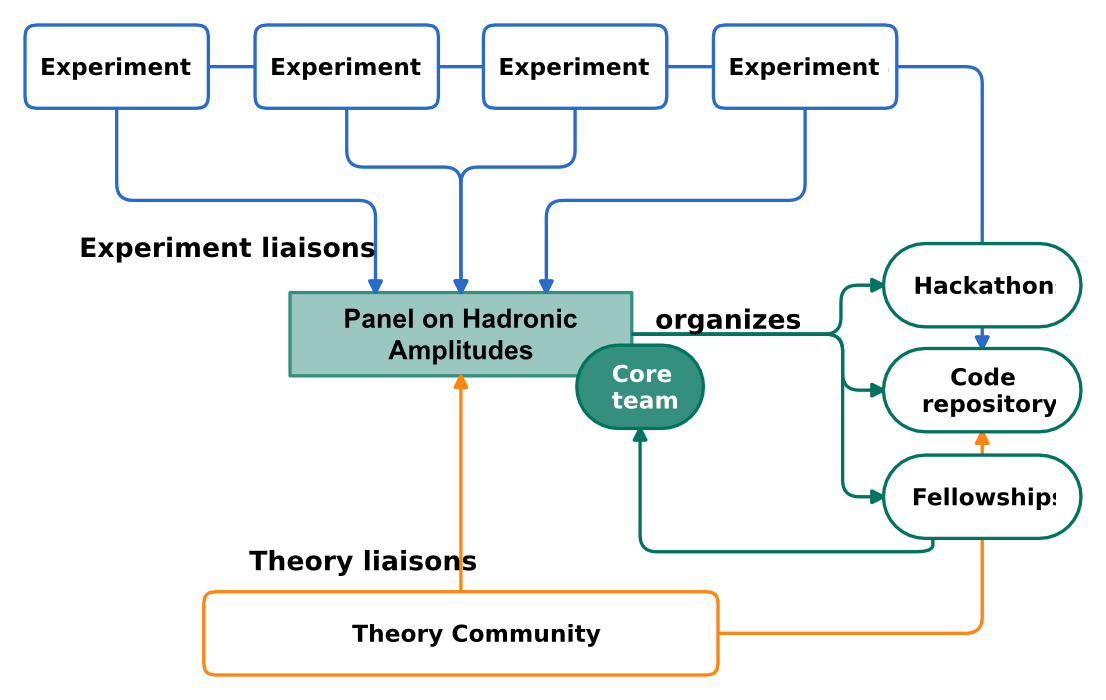
\includegraphics[width=0.8\textwidth]{PHASEstructure.png}
\end{center}

}



\frame{
\frametitle{Code-Repository as Center-Piece}
\Large
\begin{itemize}
\item Analysis \alert{code is the essence} of amplitude analysis
\vspace{3mm}
\item Need a place to publish and discuss code between experimentalists and theorists
\vspace{3mm}
\item Workshops are great, but we need to \alert{walk the walk}
\vspace{5mm}
\item \link{https://about.gitlab.com/features/}{GITLAB} is opensource and provides all features to store, develop and criticise code and its documentation 
\end{itemize}

}

\frame{
\frametitle{Role of the Panel}
\Large
\begin{itemize}
\item Ensure the \alert{flow of information} 
\item \alert{Curate} the PHASE repository
\item Ensure \alert{open access} to the repository
\item Facilitating a fair scrutiny of the contributed models
\item Regular \alert{review article} on the state of art of amplitude analyses.
\item Draft joint funding applications for the PHASE project.
\end{itemize}
}

\frame{
\frametitle{Repository Curation}
\large
\begin{center}
\begin{block}{Curation (wiktionary)}
\begin{itemize}
\item The act of curating, of \alert{organizing and maintaining} a collection of artworks or artifacts.
\vspace{3mm}
\item (archaic) The act of curing or healing.
\vspace{3mm}
\item (databases) The manual updating of information in a database.
\end{itemize}
\end{block}
\end{center}
}

\frame{
\frametitle{Making Contributions to the PHASE repository}
\Large
\begin{itemize}
\item The repository is open
\item \alert{Everybody} can and should contribute
\item In practice: Any people developing models or doing analysis
\vspace{5mm}
\item Contributions are handled through a \alert{standard process} such as the \link{https://rfc.zeromq.org/spec:42/C4/}{C4 Collective Code Construction Contract}
\vspace{5mm}
\item PHASE panel members can contribute but their main job is to curate, i.e. set up and maintain the process
\end{itemize}
}


\frame{
\frametitle{Additional Activities}
\large
Things PHASE will do:
\vspace{3mm}
\begin{itemize}
\item Organize ampltiude analysis \alert{hackathons}
\vspace{3mm}
\item Provide \alert{validation} of amplitude models
\item Award \link{https://openbadges.org/}{badges} to analyses, which meet standards of practice
\vspace{3mm}
\item Community building
\vspace{3mm}
\item Advocate for \alert{Open-Data} initiatives
\vspace{3mm}
\item PHASE fellowships
\end{itemize}
}

\frame{
\frametitle{PHASE Proposal}
\Large
\begin{itemize}
\item \link{https://www.authorea.com/users/42472/articles/136761/_show_article}{PROPOSAL Document}
\vspace{5mm}
\item {\small Latest change: removed strict response-time, replaced by "in timely fashion"}
\vspace{5mm}
\item \alert{Please update Names and Affiliations}
\end{itemize}
}

\frame{
\frametitle{Next Step: Reaching Out}
\Large
\begin{itemize}
\item Experiments to contact:\\
COMPASS, BES III, Belle, Belle II, LHCb, CLEO, BaBar, CLAS, GlueX, CB-Elsa,
 CrystalBall@MaMi, SND, CMD-3, PANDA
 \vspace{3mm}
\item List of individuals, see email
\item Open question: Meson and Baryon-communities?
\item Email to be sent on 10th of February
\vspace{3mm}
\item Session on Monday 13th at ATHOS Workshop in Bad Honeff
\end{itemize}
}


\beginbackup

\frame{
\begin{center}
\Large Backup
\end{center}
}



\frame{
\frametitle{Getting Funding: Amplitude Analysis Hackathons}
\Large
\begin{itemize}
\item Get a group of experts together for 3 weeks
\item Concrete task to implement e.g. a certain amplitude model that is needed
\item Pay for accommodation during workshop
\item Results will be made public through HAP servers
\end{itemize}
}


\frame{
\frametitle{}
\begin{center}
\Large
A pragmatic proposal\\
Amplitude Analysis Reference Library
\end{center}
}




%\frame{
%\tableofcontents
%}
\frame{
\frametitle{A Reference Implementation}
\large
\begin{itemize}
\item The purpose of the library is to implement the \alert{physics functions} needed for amplitude analysis.
\item While we will try to make it fast, optimization towards certain technologies is not the main focus of the effort.
\vspace{5mm}
\item It will become a \alert{reference implementation} 
\begin{itemize}
\item Analysers can use the library directly in their fitters
\item Comes with a \alert{test-suite} to compare custom implementations against
\end{itemize}
\item Working groups and reviewers will be able to request\\ \alert{consistency checks} against the reference library.
\vspace{5mm}
\item Goal: a \alert{consistent, tested and documented set of functions}\\ for all amplitude analyses in LHCb
\item Can be used to communicate our models to theorists
\end{itemize}
}




\frame{
\frametitle{The need to share}

\begin{itemize}
\item Parametrisations of hadronic amplitudes often quite complicated
\item Details matter 
\item Most journal formats don't allow enough space for detailed (enough) documentation
\item Best efforts in written documentation may omit important technical details 
\vspace{5mm}
\item \alert{Need a public code-base}
\end{itemize}
}


\frame{
\frametitle{Example: Plethora of implementations}
Just LHCb (3-body amplitudes, \HepProcess{\PKst\Pmu\Pmu} et al not included):
\vspace{3mm}
\begin{itemize}
\item cfit \hfill \url{https://github.com/cfit/cfit}
\item Laura++ \hfill\url{http://laura.hepforge.org/}
\item RapidFit \hfill\url{https://github.com/gcowan/RapidFit}
\item Custom fitters used for pentaquark analysis
\item Mint, Mint2, Mint3
\item Lambda\_b to OpenCharm fitter
\item Rio++
\item GPU fitter for B2Kpipi
\item GOOFit + tools \hfill\url{https://github.com/GooFit/GooFit}
\end{itemize}


}


\frame{
\frametitle{Impediments to Open-Sourcing / Standardizing}


\begin{itemize}
\item Protectionism
\begin{itemize}
\item Fear of freeloaders
\item Competitive advantage 
\end{itemize}
\vspace{3mm}
\item Not-Invented-Here syndrom
\begin{itemize}
\item Grants given for leading a project, not contributing to existing ones
\item Learning barriers of existing projects
\end{itemize}
\vspace{3mm}
\item Plurality of technical solutions
\begin{itemize}
\item Experiment specific physics (backgrounds, production mechanisms...)
\item Experiment specific software (framework integration,...)
\item Different statistical methods
\item Computing architectures (CPU clusters, GPUs, ...)
\end{itemize}
\end{itemize}

}


\frame{
\frametitle{How can we create momentum?}
{\bfseries Top down (funding agencies, collaborations):}
\begin{itemize}
\item Demand open-sourcing code/data as part of publication 
\item Better reward open-source contributions in career paths
\item Demand more journal space for complex analysis \\
(go for PRD insteadof PRL)
\end{itemize}
\vspace{5mm}
{\bfseries Bottom up (community):}
\begin{itemize}
\item Make it easy for theorists and experimentalists to contribute to same project
\item Workshops like this one!
\item Acknowledge technological plurality
\item \alert{Put code-repository at the center of efforts}
\end{itemize}
}


\backupend
\end{document}






